\section{Introduction}

% This project is an assignment by Prof. Fanucci to Mancini and Origlia.
% The purpose of the project is to practice electronics design using
% the hardware description language VHDL and Vivado, after attending the courses
% of \textit{Electronics and communications systems} at the Computer Engineering
% Master Degree Courses (for Mancini) and \textit{Microelecronics for telecommunications}
% at the Telecommunications Engineering Master Degree (for Origlia).

The assignment consists of the design of a Voice Activity Detector (VAD), a
system that takes an audio stream as input and it outputs a logical value that
indicates whether the voice is present or absent.

\subsection{Specifications}
\begin{itemize}
  \item The input stream is divided in frames of duration
  $T_{frame} = 16\si{\milli\second}$
  \item The sampling rate is $f_s = 16 \si{\kilo\hertz}$
  \item The mean frame energy is $ E_{frame} = \frac{1}{N}\sum_{n=1}^N x^2[n] $
  \item The samples range from -1 to 1: $x[n] \in [-1, 1)$
  \item The mean frame energy is compared to a given threshold:
  $ E_{threshold} = 0.05 $
  \item The input data are represented in 2 complement using 16 bits
  \item The ports of the VAD are:
  \begin{itemize}
    \item \texttt{x}: 16 bits representing the samples
    \item \texttt{FRAME\_START}: it signals the start of the frame by
    a pulse of 1 clock cycle
    \item \texttt{rst\_n}: the system active low reset
    \item \texttt{clk}: the system clock
    \item \texttt{VAD}: the output. High for \textit{voice detected},
    low otherwise.
  \end{itemize}
\end{itemize}

\begin{figure}[]
  \centering
  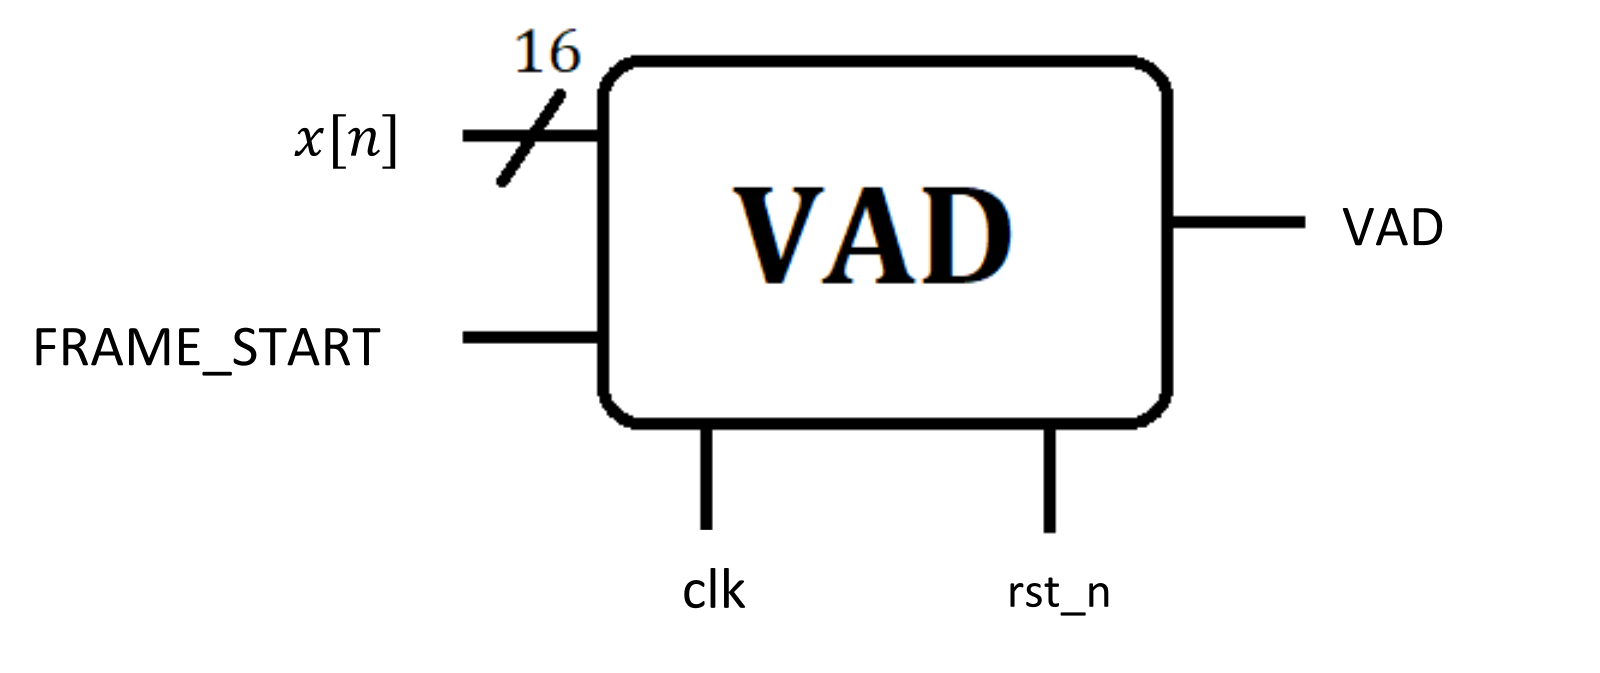
\includegraphics[width=0.75\textwidth]{figs/vad_schematic.png}
  \caption{Schematic for the VAD component}
  \label{fig:schematic}
\end{figure}
